\chapter*{Dodatak: Prikaz aktivnosti grupe}
		\addcontentsline{toc}{chapter}{Dodatak: Prikaz aktivnosti grupe}
		
		\section*{Dnevnik sastajanja}
		
		
		\begin{packed_enum}
			\item  sastanak
			
			\item[] \begin{packed_item}
				\item Datum: 16. listopada 2023.
				\item Prisustvovali: N. Ivić, M. Krajinović, M. Matulić, B. Mikan, A. Radoš, M. Žagar, I. Žinić
				\item Teme sastanka:
				\begin{packed_item}
					\item  sastanak s asistentom i demonstratorom
					\item  raspodijela zadataka 
					\item  dogovor o korištenim tehnologijama
				\end{packed_item}
			\end{packed_item}
			
			\item  sastanak
			\item[] \begin{packed_item}
				\item Datum: 19. listopada 2023.
				\item Prisustvovali: B. Mikan, A. Radoš, M. Žagar
				\item Teme sastanka:
				\begin{packed_item}
					\item  uvod u frontend tehnologije
					\item  uvod u proces razvoja frontenda
				\end{packed_item}
			\end{packed_item}
			
			\item  sastanak
			\item[] \begin{packed_item}
				\item Datum: 21. listopada 2023.
				\item Prisustvovali: N. Ivić, M. Krajinović
				\item Teme sastanka:
				\begin{packed_item}
					\item  dogovorena struktura backend dijela aplikacije
					\item  objašnjen fastapi i sqlalchemy
					\item  detaljnije dogovorena podjela posla u podtimu
				\end{packed_item}
			\end{packed_item}

			\item  sastanak
			\item[] \begin{packed_item}
				\item Datum: 23. listopada 2023.
				\item Prisustvovali: N. Ivić, M. Krajinović, M. Matulić, B. Mikan, A. Radoš, M. Žagar, I. Žinić
				\item Teme sastanka:
				\begin{packed_item}
					\item  dogovaranje detalja oko implementacije
					\item  raščišćavanje osnovnih dilema funkcionalnosti 
				\end{packed_item}
			\end{packed_item}

			\item  sastanak
			\item[] \begin{packed_item}
				\item Datum: 25. listopada 2023.
				\item Prisustvovali: M. Matulić, I. Žinić
				\item Teme sastanka:
				\begin{packed_item}
					\item  detaljnija razrada opisa zadatka
					\item  raspisivanje funkcionalnih zahtjeva i opis obrazaca uporabe
				\end{packed_item}
			\end{packed_item}
			
			\item  sastanak
			\item[] \begin{packed_item}
				\item Datum: 28. listopada 2023.
				\item Prisustvovali: B. Mikan, A. Radoš, M. Žagar
				\item Teme sastanka:
				\begin{packed_item}
					\item  diskusija oko dizajniranja sučelja u alatu figma
					\item  uvod u proces razvoja frontenda
					\item  odabir color palete
					\item  generalni apstraktni plan arhitekture aplikacije
					\item  branch naming konvencija
					\item  podijeljeni prvi jira taskovi
				\end{packed_item}
			\end{packed_item}
			
			\item  sastanak
			\item[] \begin{packed_item}
				\item Datum: 6. studenoga 2023.
				\item Prisustvovali: N. Ivić, M. Krajinović, M. Matulić, B. Mikan, A. Radoš, M. Žagar, I. Žinić
				\item Teme sastanka:
				\begin{packed_item}
					\item  rješavanje nesuglasica
					\item  daljnja raspodjela posla
					\item  dogovor oko budućih uvjeta zadatka
					\item  uvod u tehnički proces puštanja aplikacije u pogon
				\end{packed_item}
			\end{packed_item}
			
			\item  sastanak
			\item[] \begin{packed_item}
				\item Datum: 13. studenoga 2023.
				\item Prisustvovali: N. Ivić, M. Krajinović, M. Matulić, B. Mikan, A. Radoš, M. Žagar, I. Žinić
				\item Teme sastanka:
				\begin{packed_item}
					\item  organizacija puštanja aplikacije u pogon
					\item  testiranje aplikacije
					\item  provjera detalja aplikacije i dokumentacije
				\end{packed_item}
			\end{packed_item}
			
			\item  sastanak
			\item[] \begin{packed_item}
				\item Datum: 4. prosinca 2023.
				\item Prisustvovali: N. Ivić, M. Krajinović, M. Matulić, B. Mikan, A. Radoš, I. Žinić
				\item Teme sastanka:
				\begin{packed_item}
					\item  daljnja raspodjela posla
					\item  dogovori između frontenda i backenda
				\end{packed_item}
			\end{packed_item}
			
			\item  sastanak
			\item[] \begin{packed_item}
				\item Datum: 11. prosinca 2023.
				\item Prisustvovali: N. Ivić, M. Krajinović, M. Matulić, B. Mikan, A. Radoš, M. Žagar
				\item Teme sastanka:
				\begin{packed_item}
					\item  pregled grešaka prve revizije
					\item  razgovor s profesorom
					\item  planiranje budućeg rada
				\end{packed_item}
			\end{packed_item}

			\item  sastanak
			\item[] \begin{packed_item}
				\item Datum: 18. prosinca 2023.
				\item Prisustvovali: N. Ivić, M. Krajinović, M. Matulić, B. Mikan, A. Radoš, M. Žagar, I. Žinić
				\item Teme sastanka:
				\begin{packed_item}
					\item  pregled do sada obavljenog dijela
					\item  daljnja raspodjela posla
					\item  planiranje budućeg rada
				\end{packed_item}
			\end{packed_item}
			
			\item  sastanak
			\item[] \begin{packed_item}
				\item Datum: 8. siječnja 2024.
				\item Prisustvovali: N. Ivić, M. Krajinović, M. Matulić, B. Mikan, M. Žagar
				\item Teme sastanka:
				\begin{packed_item}
					\item  pregled do sada obavljenog posla
					\item  dogovor oko testiranja i deploymenta
					\item  rješavanje pitanja u vezi dokumentacije
				\end{packed_item}
			\end{packed_item}
			
			\item  sastanak
			\item[] \begin{packed_item}
				\item Datum: 15. siječnja 2024.
				\item Prisustvovali: N. Ivić, M. Krajinović, M. Matulić, B. Mikan, A. Radoš, M. Žagar, I. Žinić
				\item Teme sastanka:
				\begin{packed_item}
					\item  pregled do sada obavljenog posla
					\item  rješavanje nesuglasica
					\item  planiranje zadnjeg tjedna rada
					\item  dogovori oko prezentacije
				\end{packed_item}
			\end{packed_item}
			
			%
			
		\end{packed_enum}
		
		\eject
		\section*{Tablica aktivnosti}
		
			
			 \textit{Napomena: Doprinosi u tablici su navedeni u satima.}

			\begin{longtblr}[
					label=none,
				]{
					vlines,hlines,
					width = \textwidth,
					colspec={X[7, l]X[1, c]X[1, c]X[1, c]X[1, c]X[1, c]X[1, c]X[1, c]}, 
					vline{1} = {1}{text=\clap{}},
					hline{1} = {1}{text=\clap{}},
					rowhead = 1,
				} 
			
				\SetCell[c=1]{c}{} & \SetCell[c=1]{c}{\rotatebox{90}{\textbf{Nora Ivić}}} & \SetCell[c=1]{c}{\rotatebox{90}{\textbf{Mirta Krajinović }}} &	\SetCell[c=1]{c}{\rotatebox{90}{\textbf{Marta Matulić }}} & \SetCell[c=1]{c}{\rotatebox{90}{\textbf{Bruno Mikan }}} &	\SetCell[c=1]{c}{\rotatebox{90}{\textbf{Antonio Radoš }}} & \SetCell[c=1]{c}{\rotatebox{90}{\textbf{Marko Žagar }}} &	\SetCell[c=1]{c}{\rotatebox{90}{\textbf{Ivan Žinić }}} \\  
				Upravljanje projektom 		& 14 &  &  &  &  &  & \\ 
				Opis projektnog zadatka 	&  &  & 7 &  &  &  & 3 \\ 
				
				Funkcionalni zahtjevi       &  &  & 6 &  &  &  & 9 \\ 
				Opis pojedinih obrazaca 	&  &  & 2 &  &  &  & 6 \\ 
				Dijagram obrazaca 			&  &  &  &  &  &  & 9 \\ 
				Sekvencijski dijagrami 		&  &  & 6 &  &  &  & 1 \\ 
				Opis ostalih zahtjeva 		&  &  & 2 &  &  &  &  \\ 

				Arhitektura i dizajn sustava	 &  &  & 6 &  &  &  & 1 \\ 
				Opći prioriteti i svrha sustava  & 5 & 5 & 9 & 5 & 5 & 5 & 9 \\ 
				Dizajn baze podataka			& 3 & 12 & 2 &  &  &  &   \\ 
				Dokumentacija baze podataka	&  & 2 & 8 &  &  &  & 8  \\ 
				Dijagram razreda 			& 1 & 1 & 16 & 2 &  & 2 & 16 \\ 
				Dijagram stanja				&  &  & 1 &  &  &  & 9 \\ 
				Dijagram aktivnosti 		&  &  & 6 &  &  &  &  \\ 
				Dijagram komponenti			&  &  & 8 &  &  &  & 1 \\ 
				Korištene tehnologije i alati 		& 10 & 9 & 13 & 9 & 12 & 12 & 8 \\ 
				Ispitivanje programskog rješenja 	& 15 & 15 & 12 & 9 & 10 & 8 & 2 \\ 
				Dijagram razmještaja			&  &  &  &  &  &  & 7 \\ 
				Upute za puštanje u pogon 		& 5 &  &  & 2 &  &  & 6 \\  
				Plan rada					 & 14 & 14 & 14 & 19 & 19 & 19 & 14 \\ 
				Dnevnik sastajanja 			&  &  & 2 &  &  &  & 5 \\ 
				Zaključak i budući rad 		&  &  &  &  &  &  & 5 \\  
				Popis literature 			&  &  & 1 &  &  &  &  \\  

				Definiranje endpointa		& 6 &  &  &  &  &  &  \\ 
				Izrada baze podataka			&  & 17 &  &  &  &  &  \\ 
				Spajanje s bazom 				& 3 & 3 &  &  &  &  &  \\  
				Backend		 			& 46 & 38 &  &  &  &  & \\  
				Deployment			& 10 & 10 &  &  &  &  &  \\ 
				Dizajn izgleda aplikacije			&  &  &  & 13 & 10 & 14 &  \\  
				Implementacija izgleda			&  &  &  & 58 & 41 & 53 &\\ 
				Povezivanje s backendom			&  &  &  & 8 & 6 & 8 &\\ 
			\end{longtblr}
					
					
		\eject
		\section*{Dijagrami pregleda promjena}
		
		%unos slike
				\begin{figure}[H]
					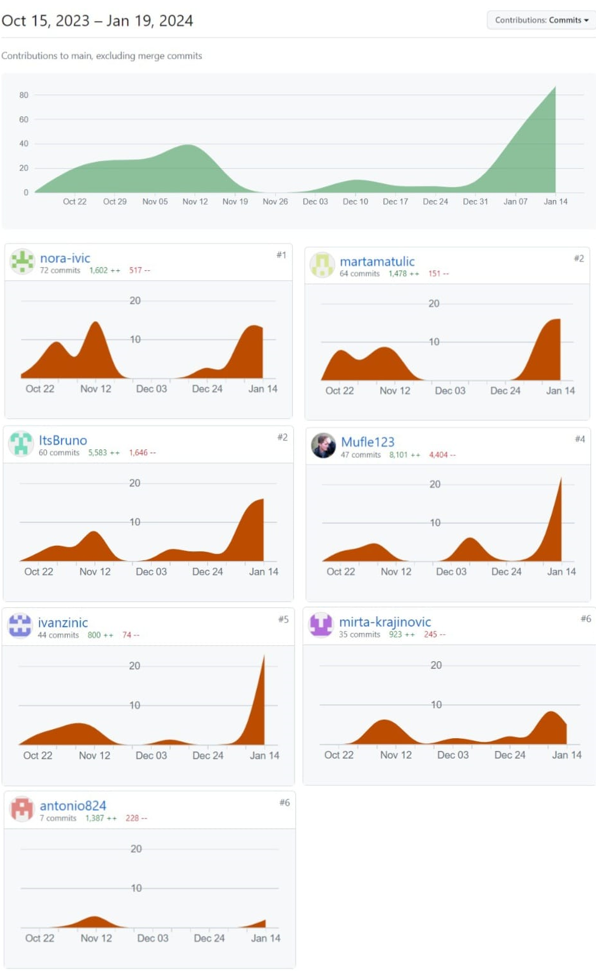
\includegraphics[scale=0.9]{slike/commitovi.PNG} %veličina slike u odnosu na originalnu datoteku i pozicija slike
					\centering
					\caption{Prikaz aktivnosti na repozitoriju}
					\label{fig:commitovi}
				\end{figure}

		
	